

\subsection{Datasets}

\noindent\textbf{KITTI3D~\cite{geiger2012we}.} KITTI 3D detection dataset consists of $7481$ images used for training, and $7518$ images used as the official \emph{test} set. We follow the standard protocol of further splitting the training set into $3712$ and $3769$ images \cite{}, and denote them by \emph{train} and \emph{val}, respectively. We perform all ablative analysis in Sec.~\ref{ablative}  by training on \emph{train} set and evaluating on \emph{val} set. The standard metrics of KITTI benchmark consist of per-class average precision (\emph{AP}) computed with thresholds on intersection-over-union (\emph{IoU}) of 3D boxes and Bird-Eye-View (2D) boxes. In order to evaluate multiclass detectors in Sec.~\ref{ablative}, we additionally use mean average precision (\emph{mAP}) by computing the average of per-class APs, as in recently introduced datasets \cite{caesar2020nuscenes, gahlert2020cityscapes}.  When reporting results on the benchmark, we train on combined set of \emph{train} and \emph{val}, and perform cross-validation with 80/20 splits.

\noindent\textbf{KITTI-depth~\cite{geiger2013vision}.} We report depth estimation results on the standard KITTI depth estimation benchmark. We follow the training protocol of Eigen et al.~\cite{eigen2014depth}, i.e. the KITTI Eiten train and test splits containing $22600$ and $697$ test images. For a fair comparison with the current state-of-the-art~\cite{ma2019accurate,fu2018deep} we report our metrics by comparing against the improved groudtruth LiDAR depth maps introduced in~\cite{geiger2013vision}. As described in Sec~\ref{subsubsec:monodepth}, we generate a new split by removing Eigen train images that overlap (spatially within 50 meters) with the KITTI3D images; we denote this split by \textit{Eigen clean} and mention that for 3D detection the depth networks are finetuned on Eigen clean and \textbf{not on} Eigen train, as has been the standard practice until recently~\cite{simonelli2020demystifying}. We thus avoid contaminating our detection results due to the depth networks overfitting on KITTI3D train/val and exhibiting poor generalization to KITTI3D test. We demonstrate the difference in 3D detection metrics when using Eigen train vs Eigen clean for depth training in the supplementary.

\noindent\textbf{CityScapes3D~\cite{gahlert2020cityscapes}.} CityScapes 3D consists of $5000$ images of urban scenes, split into $2975$ images for training, $500$ for validating, and $1525$ for testing. It is tailored for monocular 3D detection, in that the ground-truth 3D bounding box annotations are obtained using stereo imagery, and therefore avoids annotation artifacts due to parallax and synchronization error with respect to the Lidar sensor. The detection benchmark requires to report 3D bounding boxes of 6 vehicle types. The evaluation metric, \emph{mean detection score} (\emph{mDS}), is computed as the average four depth-dependent metrics measuring errors in predicted center distance, orientation, and size, weighted by 2D detection metric (\emph{AP}).

\noindent\textbf{nuScenes~\cite{caesar2020nuscenes}.} nuScenes dataset consists of $1000$ multimodal videos with full $360$-degree field of view, capturing urban areas of Boston and Singapore from 6 cameras and Lidar / Radar devices. The videos are split into $700$ videos for training, $150$ for validating, and $150$ for testing. The 3D detection benchmark requires to report 3D bounding boxes of 10 object classes over 2Hz-sampled video frames of 360-degree view. The evaluation metric, \emph{nuScenes detection score} (\emph{NDS}), is computed by combining detection accuracy (\emph{mAP}) computed over four different thresholds on center distance with five true-positive metrics. Among them, we only consider three metrics that concerns 3D detection, i.e. \emph{ATE}, \emph{ASE}, and \emph{AOE}.

\noindent\textbf{Depth pretraining.} To pretrain our models, we build a large-scale internal dataset that contains monocular videos and accurate ground-truth depth captured from high-resolution Lidar devices across a full 360-degree field of view. It pictures urban scenes in various cities of US and Japan. We randomly subsample $1K$, $5K$, $10K$, and $25K$ videos (10 seconds each), and refer to these datasets as \textbf{Pretrain-[1k, 5k, 10k, 25k]}, respectively.

\subsection{Implementation}
\label{implementation}
\noindent\textbf{Depth pretraining.} 

\noindent\textbf{Pseudo-Lidar.}

\noindent\textbf{FCOS-3D.}

%\subsection{Depth estimation.}
 

%\noindent\textbf{Pretraining.}
%To quantify the effect of depth quality we pretrain our depth estimation networks on a large internal dataset consisting of image and LiDAR pairs. The complete dataset consists of 25K scenes, each scene being captured with a frequency of $10Hz$ over $10$ seconds, for a total of 25M image + LiDAR pairs. We randomly subsample 1K, 5K and 10K scenes from the complete scene set, and generate a total of 4 pretraining splits (including the complete dataset); for brevity, we will refer to these splits as \textbf{1K}, \textbf{5K}, \textbf{10K} and \textbf{25K} whenever appropriate. Importantly, the downsampled splits contain fewer images as well as less diversity, as we downsample from the scene set and not from the image set. We use the generated splits for pre-training the depth networks, and we perform experiments that estimate depth quality vs. 3D detection performance at each pretraining level. We describe the pretraining protocol in detail in the supplementary. 

% and mention that we ensured that each model is trained to convergence. 


% \subsection{FCOS-3D}
% \textbf{Pretraining backbone}
% \begin{figure}[t]
% 	\centering
% 	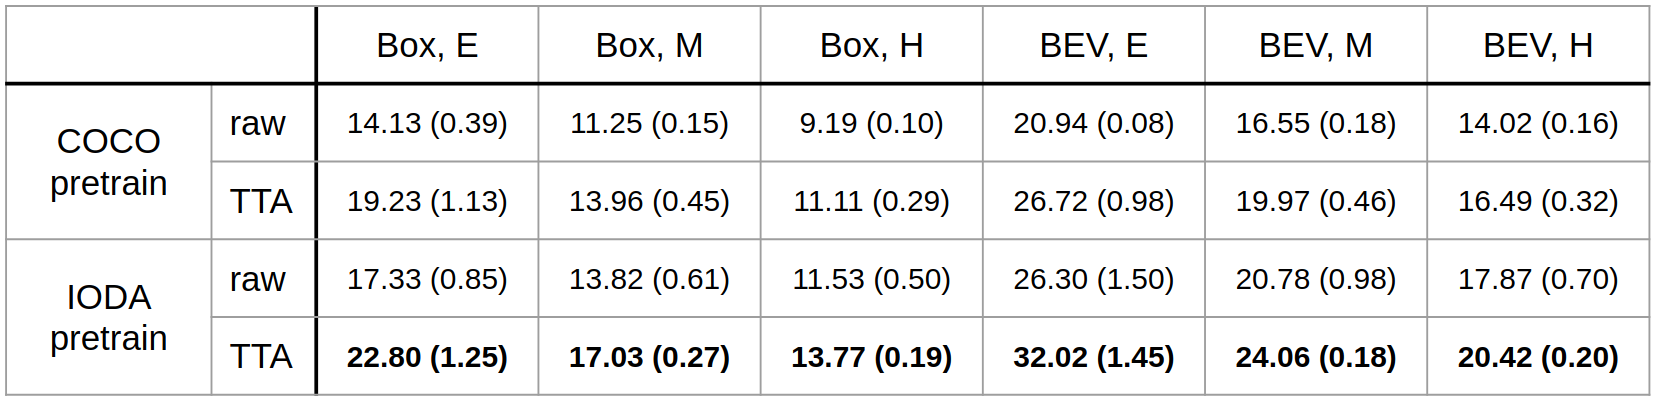
\includegraphics[width=1.0\columnwidth]{figures/fcos3d_backbone_pretrained.png}
% \end{figure}
